\documentclass[a4paper,12pt,reqno]{article}

% --------------------------------------------------------
% Packages
% --------------------------------------------------------
\usepackage[utf8]{inputenc}
\usepackage{mathtools,graphicx}
\usepackage[colorlinks=true, allcolors=blue]{hyperref}
\usepackage{amsmath,amsfonts,amssymb,amsthm,mathrsfs,bm}
\usepackage[margin=0.95in]{geometry}
\usepackage{setspace}
\usepackage[table,xcdraw]{xcolor}
\usepackage{float} % 支持图片浮点嵌入 e.g.,\begin{figure}[H]
\usepackage{subfigure} % 支持多图
\usepackage{cite}
\usepackage{siunitx} % 支持各类正体单位 e.g.,\unit{\kg}(建议在数字和单位间插入\,以留出适当间隙)
\usepackage{txfonts} % 支持正体希腊字母 e.g.,$\muup$ 注:添加该包会对默认字体有影响
\usepackage{url} % bibTex支持引用网页

% --------------------------------------------------------
% Custom Commands
% --------------------------------------------------------
% \renewcommand{\rmdefault}{phv} % Arial
% \renewcommand{\sfdefault}{phv} % Arial
\renewcommand\thesection{\arabic {section}} % Section numbers start from 1
% \renewcommand{\bibname}{References}
\newcommand{\HRule}{\rule{\linewidth}{0.5mm}}
\DeclareUnicodeCharacter{2212}{-}

% --------------------------------------------------------
% Opening: Title and Author Names
% --------------------------------------------------------
% \begin{document}

% \textsc{
%     \vspace{-3cm}
%     \begin{center}
%         \center\LARGE Queen's University Belfast \\[0.5cm]
%         \Large ELE8096 Wireless Sensor Systems \\[0.5cm]
%     \end{center} 
% }
% \textsc{
%     % \vspace{-1cm}
%     \begin{flushleft}
%         \Large Coursework1 \hfill
%         \small Student: Name \ Student Number: 12345678
%     \end{flushleft}
% }
\begin{document}

\textsc{
    \vspace{-3cm}
    \begin{center}
        \center\LARGE Queen's University Belfast \\[0.5cm]
        \Large ELE8096 Wireless Sensor Systems \\[0.5cm]
    \end{center} 
}
\textsc{
    % \vspace{-1cm}
    \begin{flushleft}
        \Large Coursework1 \hfill
        % \small Student: \ \ \ \ \ \ Zichi Zhang \ Student Number: 40299571\\
        % \hfill Muzixiang Xiao \, \ \ \ \ \ \ \ \ \ \ \ \ \ \ \ \ \ \ \ \ \ \ \ \ \ \ \ \ \ 40344034\\
        % \hfill Jiyu Zou \, \ \ \ \ \ \ \ \ \ \ \ \ \ \ \ \ \ \ \ \ \ \ \ \ \ \ \ \ \ 40344034\\
        % \hfill Yuhang Zhang \, \ \ \ \ \ \ \ \ \ \ \ \ \ \ \ \ \ \ \ \ \ \ \ \ \ \ \ \ \ 40344034\\
        % \hfill Chuao Zheng \, \ \ \ \ \ \ \ \ \ \ \ \ \ \ \ \ \ \ \ \ \ \ \ \ \ \ \ \ \ 40344034\\
        % \hfill Yujie Yang \, \ \ \ \ \ \ \ \ \ \ \ \ \ \ \ \ \ \ \ \ \ \ \ \ \ \ \ \ \ 40344034
        \large Group: 5
    \end{flushleft}
}
% --------------------------------------------------------
% Section 1: Group Task – Data Set and Basic Statistics
% --------------------------------------------------------
\vspace{-0.5cm}
\section*{Part II: Group Task – Data Set and Basic Statistics}\label{sec:1}
    Write something here.

% Subsection: Identifying a Data Set
% ^^^^^^^^^^^^^^^^^^^^^^^^^^^
\vspace{-0.5cm}
\subsection*{Identifying a Data Set}
    We build a Github Repositorie and upload the data set, it is public to check from this link:
    \href{https://github.com/Gczmy/ELE8096/blob/main/Coursework1_Group_Part/NO2_DATA.xlsx}{The Data Set}. 
    And the data source is from the UK AIR Air Information Resource, it can be check with some steps from this link:
    \href{https://uk-air.defra.gov.uk/data/datawarehouse}{The Data Source}.\\

% Subsection: Background on the importance of pollutant and legislation on thresholds
% ^^^^^^^^^^^^^^^^^^^^^^^^^^^
\vspace{-0.5cm}
\subsection*{Background on the importance of pollutant and legislation on thresholds}
    Nitrogen Dioxide (NO$_2$) is one of a group of 
    highly reactive gases known as oxides of nitrogen 
    or nitrogen oxides (NO$_{\mathrm{x}}$). Other 
    nitrogen oxides include nitrous acid and nitric 
    acid. NO$_2$ is used as the indicator for the 
    larger group of nitrogen oxides. 
    NO$_2$ primarily gets in the air from the burning of fuel. 
    NO$_2$ forms from emissions from cars, trucks and buses, 
    power plants, and off-road equipment.
    \paragraph{Health effects of NO$_2$:}
    Breathing air with a high concentration of NO$_2$ can irritate airways in the human respiratory system. Such exposures over short periods can aggravate respiratory diseases, particularly asthma, leading to respiratory symptoms (such as coughing, wheezing or difficulty breathing), hospital admissions and visits to emergency rooms. Longer exposures to elevated concentrations of NO$_2$ may contribute to the development of asthma and potentially increase susceptibility to respiratory infections. People with asthma, as well as children and the elderly are generally at greater risk for  the health effects of NO$_2$.
    NO$_2$ along with other NO$_{\mathrm{x}}$ reacts with other chemicals in the air to form both particulate matter and ozone. Both of these are also harmful when inhaled due to effects on the respiratory system.
    Learn more about Particulate Matter and Ozone.



% Subsection: Basic statistics on the data set
% ^^^^^^^^^^^^^^^^^^^^^^^^^^^
\vspace{-0.5cm}
\subsection*{Basic statistics on the data set}
    The figures of 12 months average duiring this year are showed below 
    as Figure \ref{fig:12_months_average_duiring_this_year}:
    \begin{figure}[H]
        \centering
        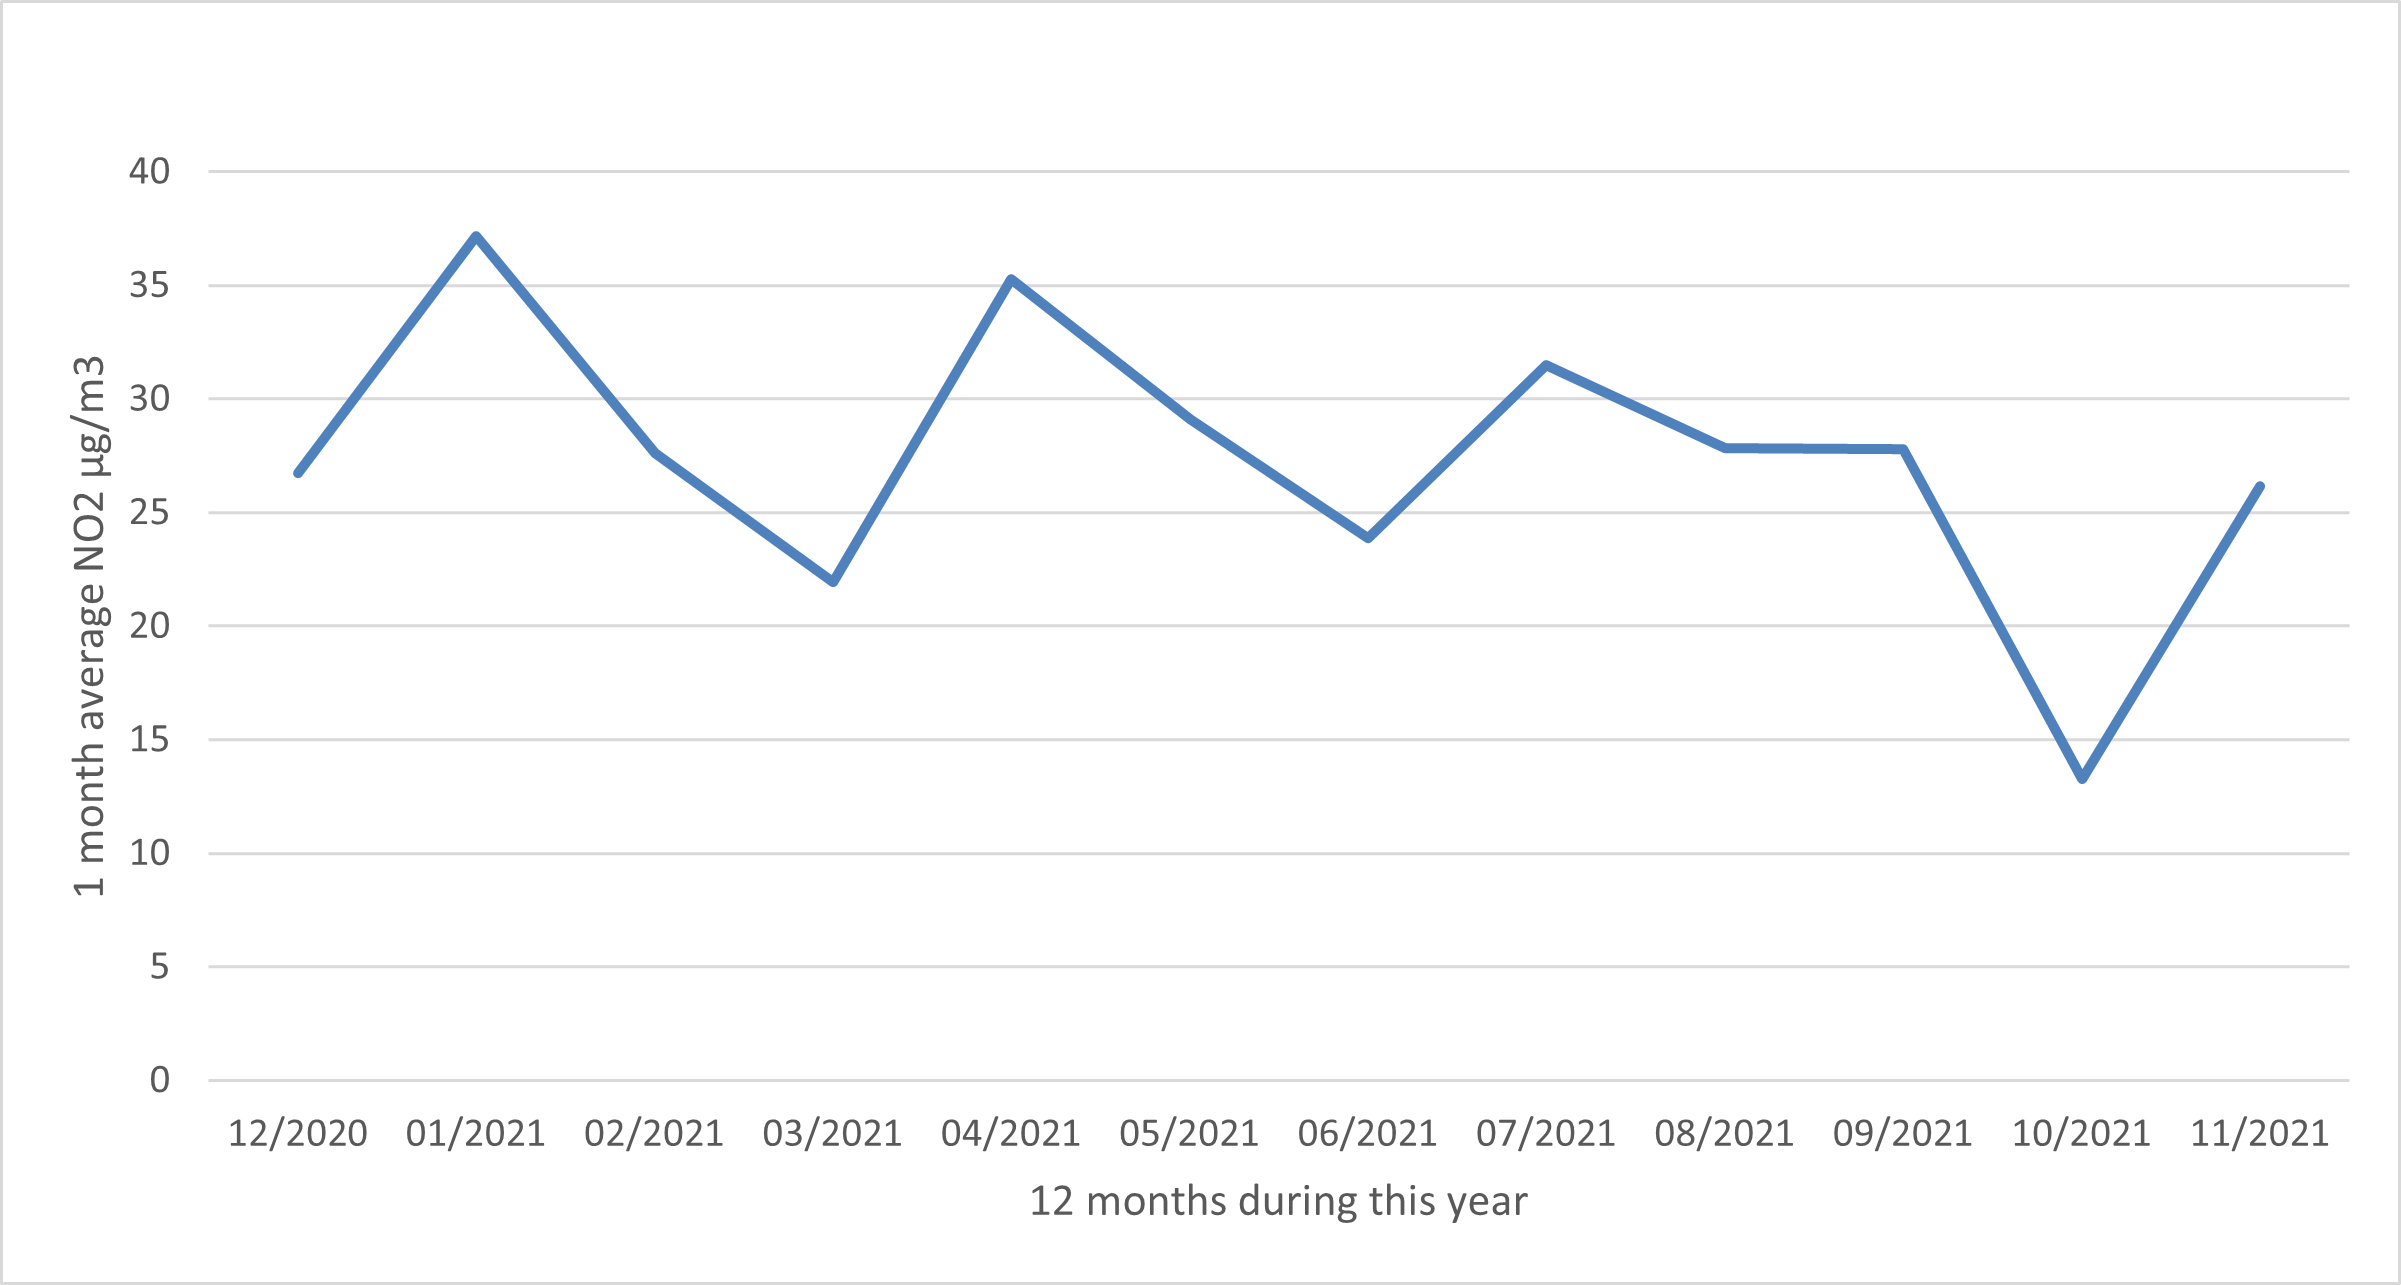
\includegraphics[width=0.7\textwidth]{figures/figure1.png}
        \caption{12 months average duiring this year}
        \label{fig:12_months_average_duiring_this_year}
    \end{figure}
    The figures of 4 season 15th comparison are showed below 
    as Figure \ref{fig:4_season_15th_comparison}:
    \begin{figure}[H]
        \centering
        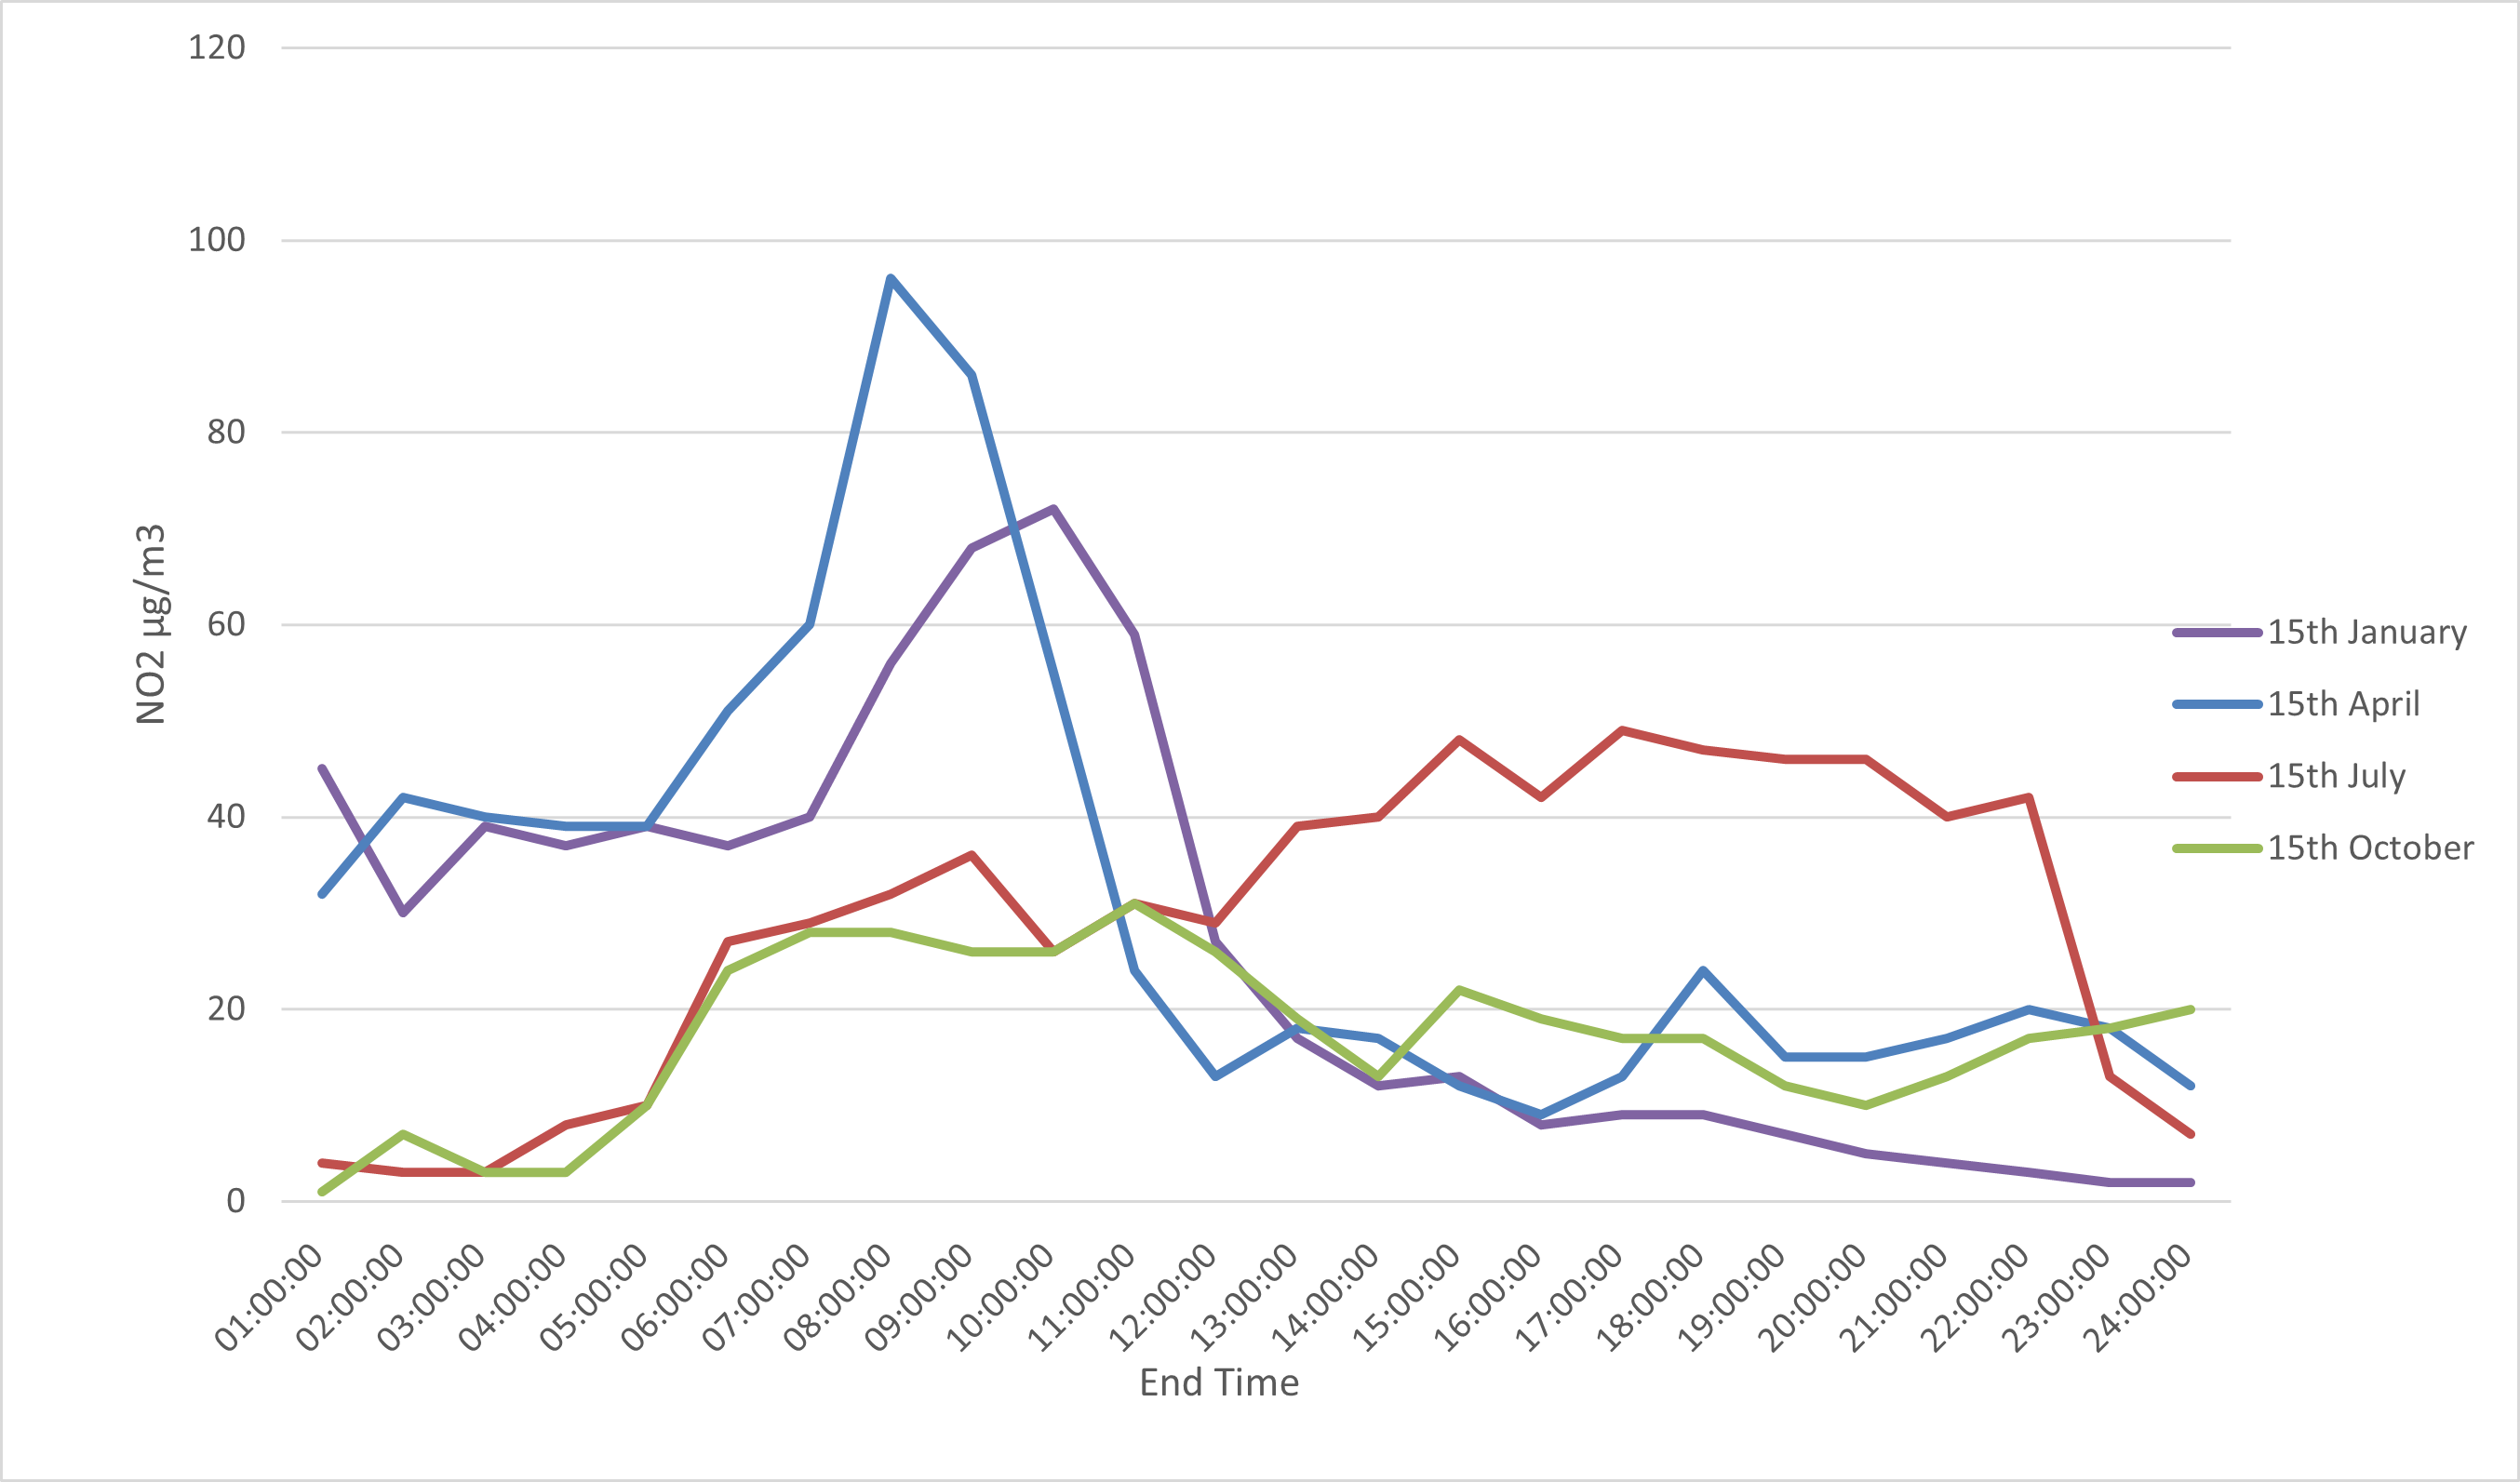
\includegraphics[width=0.7\textwidth]{figures/figure2.png}
        \caption{4 season 15th comparison}
        \label{fig:4_season_15th_comparison}
    \end{figure}

\end{document}
